\begin{tikzpicture}[
>=Stealth,
font=\sffamily\small,
box/.style={draw=black!70, rounded corners=3pt, thick, fill=white, align=center},
iconbox/.style={draw=none, fill=none, align=center, inner sep=1pt},
videobox/.style={draw=blue!60!black, rounded corners=3pt, thick, fill=black!2, align=center, inner sep=2.5pt},
framebox/.style={draw=teal!60!black, rounded corners=3pt, thick, fill=white, align=center, inner sep=2.5pt},
stepbox/.style={box, fill=green!12, draw=green!60!black, thick, font=\sffamily\scriptsize, align=center},
detector/.style={box, fill=cyan!10, draw=cyan!70, font=\sffamily\footnotesize, text width=2.6cm, minimum height=1.15cm},
fusion/.style={box, fill=purple!10, draw=purple!70, thick, font=\sffamily\footnotesize, text width=2.5cm, minimum height=1.1cm},
method/.style={box, fill=orange!10, draw=orange!75, thick, font=\sffamily\scriptsize, text width=3.7cm, inner ysep=5pt, inner xsep=7pt},
decision/.style={box, fill=teal!12, draw=teal!70, thick, font=\sffamily\footnotesize, text width=2.2cm, minimum height=1.05cm},
eval/.style={box, fill=green!10, draw=green!60!black, thick, font=\sffamily\scriptsize, text width=3.4cm, inner ysep=4.5pt, inner xsep=5pt},
kpi/.style={draw=red!70!black, fill=red!5, rounded corners=4pt, thick, align=center, inner ysep=4.5pt, inner xsep=5pt, text width=3.2cm},
arrow/.style={->, thick, draw=black!75},
bluearrow/.style={->, thick, draw=blue!70!black},
orangearrow/.style={->, thick, draw=orange!80!black},
greenarrow/.style={->, thick, draw=green!60!black},
purplearrow/.style={->, thick, draw=purple!80!black},
sig/.style={font=\fontsize{5.8pt}{6.8pt}\selectfont\bfseries, text=black},
ttl/.style={font=\fontsize{6.2pt}{7.2pt}\selectfont\bfseries}
]

% =========================================================================
% TOP SECTION: SYNTHETIC GENERATION, DUAL CROP & ANNOTATION
% =========================================================================

% 1. RGB video prompt
\node[iconbox] (prompt_rgb) at (-4.6, 6.10) {

\includegraphics[height=0.76cm]{figures/icon_lorem_ipsum.png}
};
\node[above=4pt of prompt_rgb, ttl, text=blue!80!black] (lbl_p1) {Scenario Prompt};
\node[below=2pt of prompt_rgb, font=\fontsize{5.3pt}{6.4pt}\selectfont\bfseries, text=black] (sub_p1) {Structured Text};

% 2. Video Generator LLMs
\node[iconbox] (grok_rgb) at (-1.4, 7.35) {

\includegraphics[height=0.72cm]{figures/grok_logo.png}
};
\node[above=3pt of grok_rgb, ttl, text=purple!80!black] (lbl_g1) {AI Video Generator};
\node[below=2pt of grok_rgb, font=\fontsize{5.3pt}{6.4pt}\selectfont\bfseries, text=black] (sub_grok) {xAI Grok};

\node[iconbox] (gemini_rgb) at (-1.4, 4.85) {

\includegraphics[height=0.72cm]{figures/gemini_logo.png}
};
\node[below=2pt of gemini_rgb, font=\fontsize{5.3pt}{6.4pt}\selectfont\bfseries, text=black] (sub_g1) {Google Gemini 3.8 Flash};

\draw[bluearrow] (prompt_rgb.east) -- (grok_rgb.west);
\draw[bluearrow] (prompt_rgb.east) -- (gemini_rgb.west);

% 3. 16:9 RGB Videos — Snow only in video boxes
\node[videobox] (grok_videos) at (2.6, 7.35) {
\begin{tabular}{@{}c@{\hspace{3pt}}c@{\hspace{3pt}}c@{}}
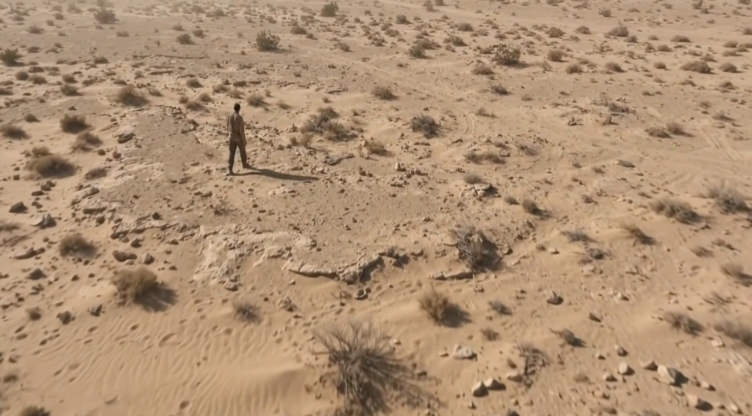
\includegraphics[width=1.12cm]{figures/grok_desert_video.png} &
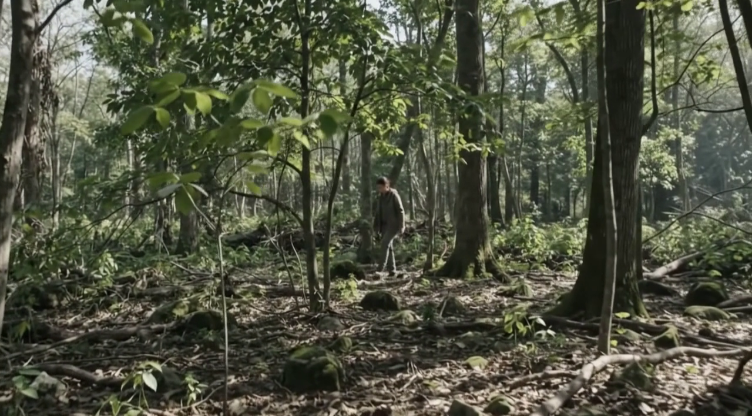
\includegraphics[width=1.12cm]{figures/grok_forest_video.png} &
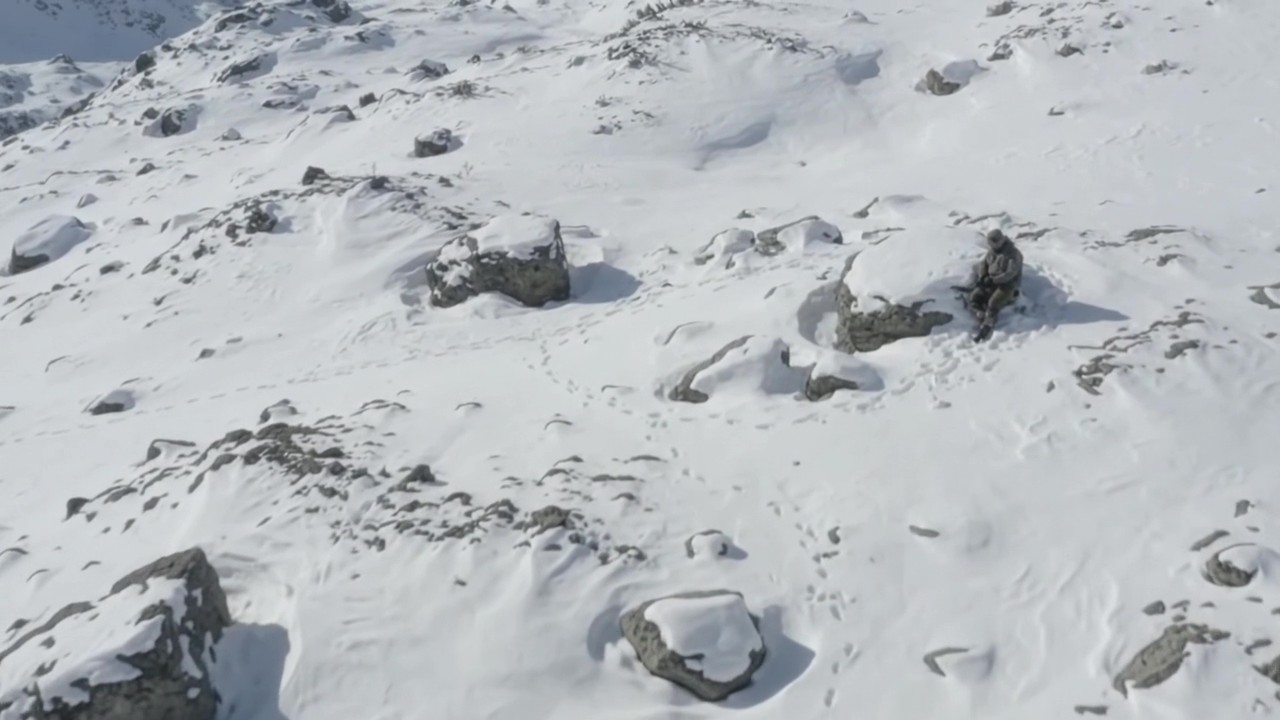
\includegraphics[width=1.12cm]{figures/snow_rgb_video.jpg} \\
{\tiny\bfseries Desert RGB} & {\tiny\bfseries Forest RGB} & {\tiny\bfseries Snow RGB}
\end{tabular}
};
\node[above=3pt of grok_videos, ttl, text=black] (lbl_gv) {16:9 RGB Videos};
\node[below=2pt of grok_videos, font=\fontsize{5.3pt}{6.4pt}\selectfont\bfseries, text=black] (sub_gv) {752$\times$416 @ 24 FPS};

\draw[bluearrow] (grok_rgb.east) -- (grok_videos.west);

\node[videobox] (rgb_videos) at (2.6, 4.85) {
\begin{tabular}{@{}c@{\hspace{3pt}}c@{\hspace{3pt}}c@{}}
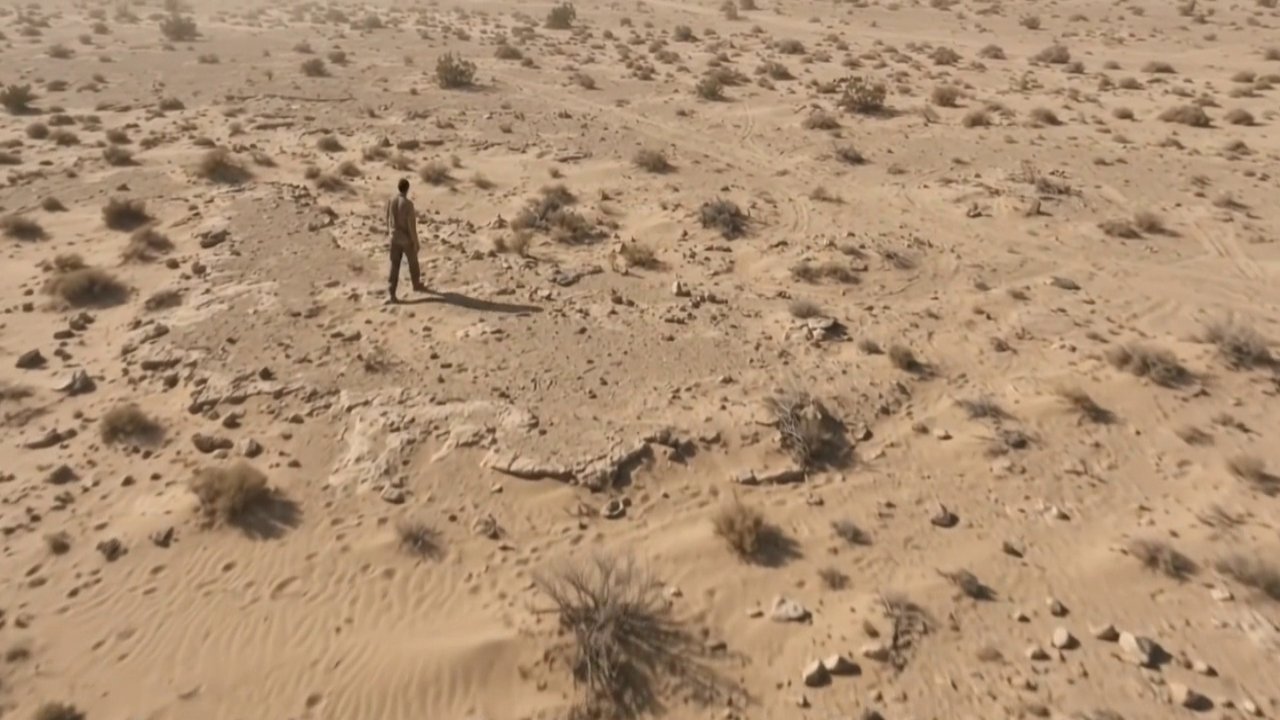
\includegraphics[width=1.12cm]{figures/desert_rgb_video.png} &
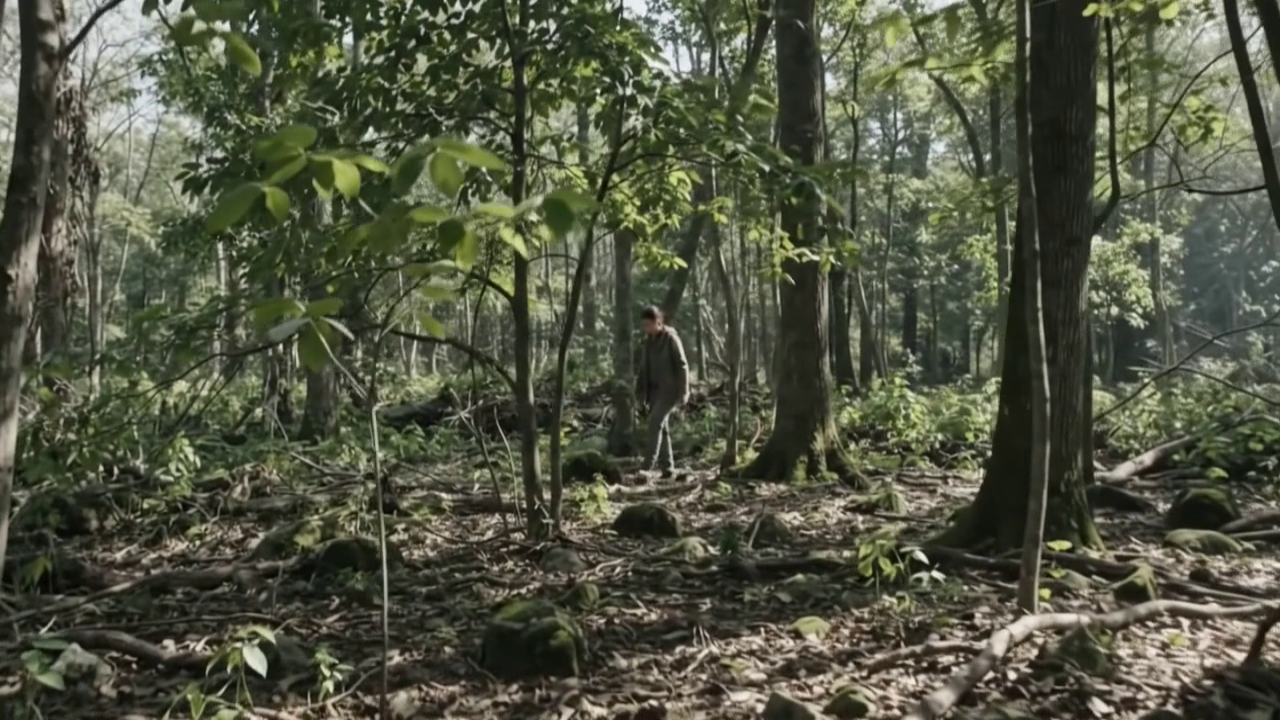
\includegraphics[width=1.12cm]{figures/forest_rgb_video.png} &
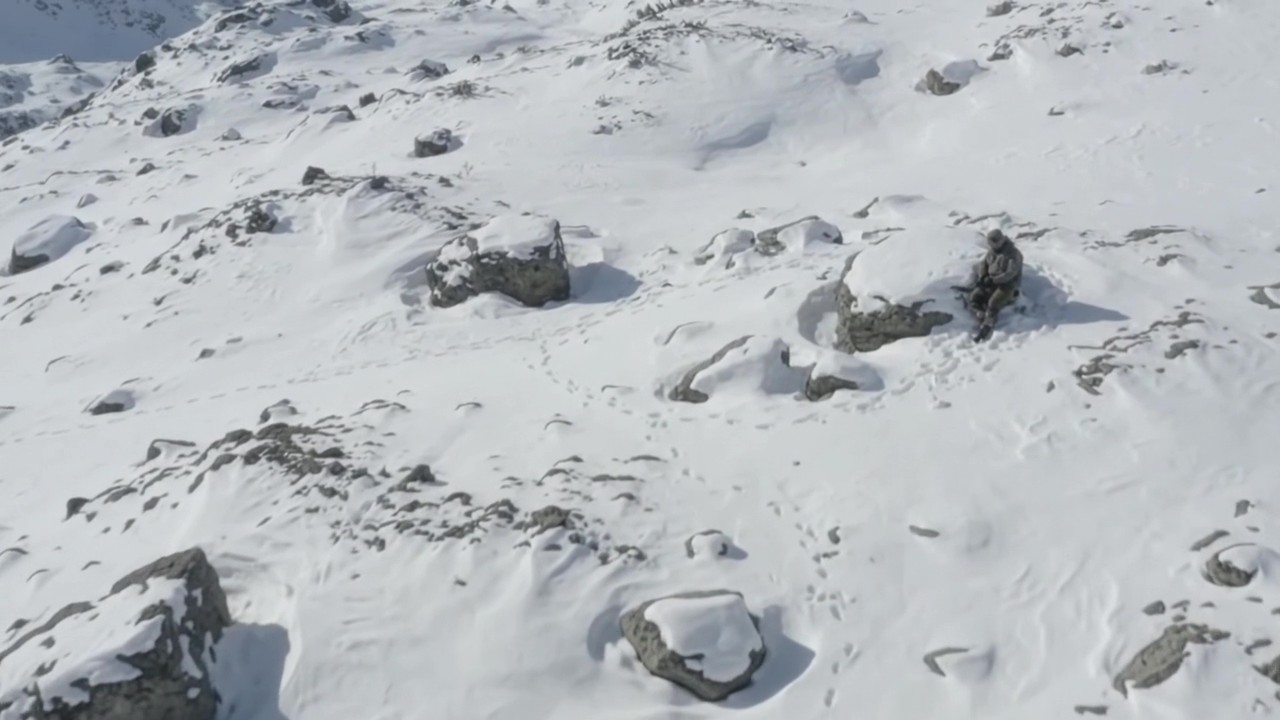
\includegraphics[width=1.12cm]{figures/snow_rgb_video.jpg} \\
{\tiny\bfseries Desert RGB} & {\tiny\bfseries Forest RGB} & {\tiny\bfseries Snow RGB}
\end{tabular}
};
\node[above=3pt of rgb_videos, ttl, text=black] (lbl_v1) {16:9 RGB Videos};
\node[below=2pt of rgb_videos, font=\fontsize{5.3pt}{6.4pt}\selectfont\bfseries, text=black] (sub_v1) {1280$\times$720 @ 24 FPS};

\draw[bluearrow] (gemini_rgb.east) -- (rgb_videos.west);

% 4. Resolution Upscale
\node[box, fill=blue!8, draw=blue!70!black, thick, font=\fontsize{5.6pt}{6.6pt}\selectfont, text width=2.1cm, align=center, minimum height=1.05cm] (upscale_box) at (6.6, 7.35) {
\textbf{Upscale to}\\[1pt]
\textbf{1280$\times$720}\\[2pt]
{\tiny Spatial Scaling}
};
\node[above=3pt of upscale_box, ttl, text=blue!80!black] (lbl_up) {Resolution Upscale};

\draw[bluearrow] (grok_videos.east) -- (upscale_box.west);

% 5. Melo Thermal Stylizing
\node[box, fill=orange!10, draw=orange!80!black, thick, font=\fontsize{5.6pt}{6.6pt}\selectfont, text width=2.6cm, align=center, minimum height=1.15cm] (melo_th) at (10.0, 6.0) {
\textbf{256-Level Color LUT}\\[2pt]
{\scriptsize Grayscale-to-TIR Remap}\\[1pt]
{\tiny Synthetic TIR Emulation}
};
\node[above=4pt of melo_th, ttl, text=orange!80!black] (lbl_melo) {Pseudo-Thermal Transfer};
\node[below=3pt of melo_th, font=\fontsize{5.3pt}{6.4pt}\selectfont\bfseries, text=black] (sub_melo) {LUT Color Mapping};

\draw[orangearrow] (upscale_box.east) -- ([yshift=5pt]melo_th.west);
\draw[orangearrow] (rgb_videos.east) -- ([yshift=-5pt]melo_th.west);

% 6. 16:9 Thermal Videos
\node[videobox] (th_videos) at (14.5, 6.0) {
\begin{tabular}{@{}c@{\hspace{3pt}}c@{\hspace{3pt}}c@{}}
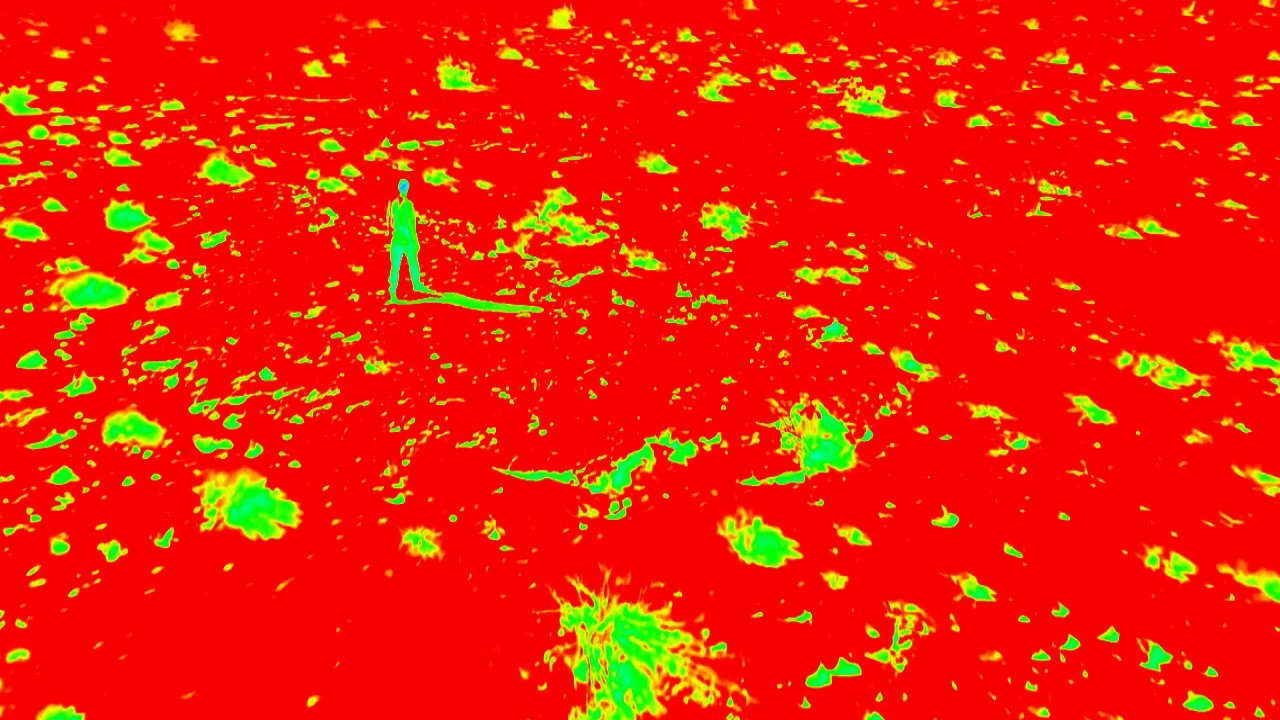
\includegraphics[width=1.12cm]{figures/desert_th_video.png} &

\includegraphics[width=1.12cm]{figures/forest_th_video.png} &

\includegraphics[width=1.12cm]{figures/snow_th_video.jpg.png} \\
{\tiny\bfseries Desert TIR} & {\tiny\bfseries Forest TIR} & {\tiny\bfseries Snow TIR}
\end{tabular}
};
\node[above=4pt of th_videos, ttl, text=black] (lbl_v2) {16:9 Thermal Videos};
\node[below=2pt of th_videos, font=\fontsize{5.3pt}{6.4pt}\selectfont\bfseries, text=black] (sub_v2) {1280$\times$720 @ 24 FPS};

\draw[orangearrow] (melo_th.east) -- (th_videos.west);

% 7. Crop 640x640
\node[videobox] (crops) at (18.5, 6.0) {
\begin{tabular}{@{}c@{\hspace{3pt}}c@{}}
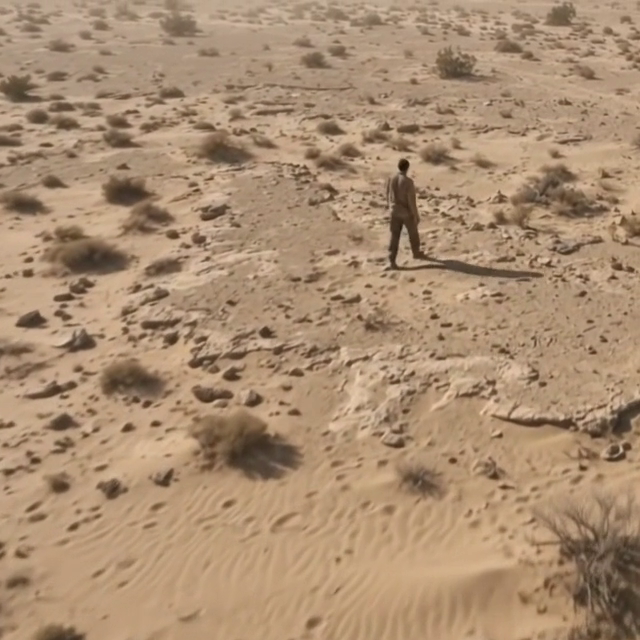
\includegraphics[width=0.83cm]{figures/crop_640_left_video.png} &

\includegraphics[width=0.83cm]{figures/crop_640_right_video.png} \\
{\tiny\bfseries Left ($x=0$)} & {\tiny\bfseries Right ($x=640$)}
\end{tabular}
};
\node[above=4pt of crops, ttl, text=purple!80!black] (lbl_c) {Crop 640$\times$640 (2 Videos)};
\node[below=2pt of crops, font=\fontsize{5.3pt}{6.4pt}\selectfont\bfseries, text=black] (sub_c) {Cropped Videos (24 FPS)};

\draw[purplearrow] (th_videos) -- (crops);

% 8. Label Studio
\node[iconbox] (label_studio) at (21.6, 6.0) {

\includegraphics[height=0.76cm]{figures/icon_label_studio.png}
};
\node[above=4pt of label_studio, ttl, text=red!80!black] (lbl_ls) {Label Studio};
\node[below=2pt of label_studio, font=\fontsize{5.3pt}{6.4pt}\selectfont\bfseries, text=black] (sub_ls) {Video Annotation};

\draw[purplearrow] (crops) -- (label_studio);

% 9. Video to Frame
\node[stepbox, text width=1.95cm, inner xsep=3pt, minimum height=1.15cm] (v2f) at (24.2, 6.0) {
\textbf{Video to Frame}\\[2pt]
{\scriptsize Full-Rate Stream}\\[-1pt]
{\scriptsize (24~Hz Sampling)}
};
\node[below=2pt of v2f, font=\fontsize{5.3pt}{6.4pt}\selectfont\bfseries, text=black] (sub_v2f) {Frame Extraction};

\draw[greenarrow] (label_studio) -- (v2f);

% 10. Annotated Frames — NO Snow RGB
\node[framebox] (annotated_frames) at (28.0, 6.0) {
\begin{tabular}{@{}c@{\hspace{3pt}}c@{\hspace{3pt}}c@{}}

\includegraphics[width=0.82cm]{figures/desert_rgb_annotated.png} &

\includegraphics[width=0.82cm]{figures/desert_th_annotated.png} &
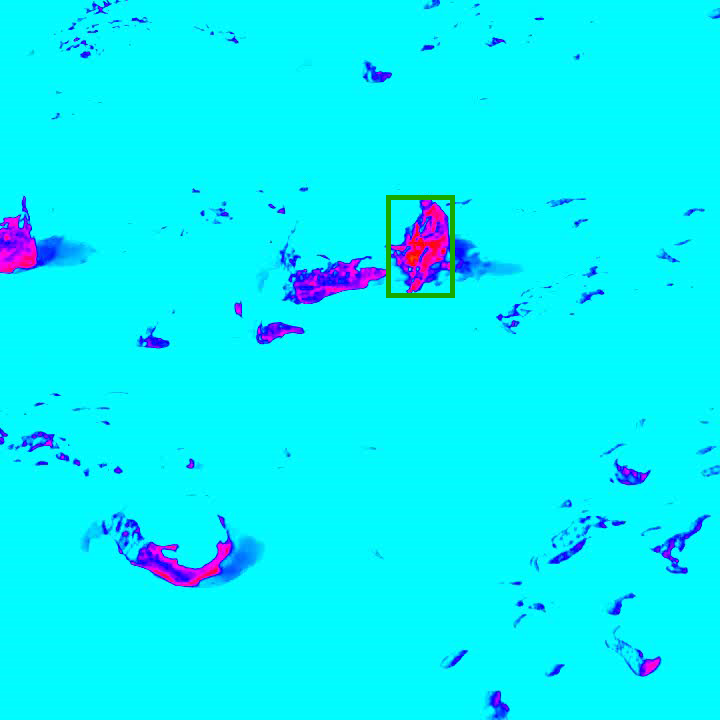
\includegraphics[width=0.82cm]{figures/snow_th_annotated.png} \\
{\tiny\bfseries RGB Frame} & {\tiny\bfseries Thermal Frame} & {\tiny\bfseries Snow TIR}
\end{tabular}
};
\node[above=4pt of annotated_frames, ttl, text=teal!80!black] (lbl_af) {Annotated Frames};
\node[below=2pt of annotated_frames, font=\fontsize{5.3pt}{6.4pt}\selectfont\bfseries, text=black] (sub_af) {Dataset Frames};

\draw[greenarrow] (v2f) -- (annotated_frames);

% =========================================================================
% MIDDLE SECTION: DATASET BANNER
% =========================================================================

\node[draw=purple!70, fill=purple!6, rounded corners=4pt, thick, font=\fontsize{5.8pt}{7.0pt}\selectfont, text=black, inner ysep=4pt, inner xsep=10pt, align=center] (dataset_banner) at (13.5, 3.65) {
\textbf{\textcolor{purple!90!black}{Benchmark Corpus and Sequence Partitioning (Option B)}}\\[2pt]
Parent-Video Grouped Split (44/22/24 tiles $\approx$ 49\%/24\%/27\%) $|$ Co-Located Left and Right Tiles\\
240 Frames/Episode at 24~Hz ($0 \to 239$ Sequential) $|$ Seed 0 Shuffled with Anti-Adjacency
};

\draw[thick, draw=purple!80, ->] (annotated_frames.east) -- ++(0.5, 0) |- (dataset_banner.east);

% =========================================================================
% BOTTOM SECTION: DETECTION, FUSION & POST-PROCESSING
% =========================================================================

\node[box, fill=purple!10, draw=purple!75, thick, font=\fontsize{5.2pt}{6.4pt}\selectfont, text width=1.9cm, align=center] (split_box) at (-1.0, -0.7) {
\textbf{Corpus Split}\\[1pt]
\textbf{Dispatch}\\[2pt]
{\scriptsize Option B Partition}\\[1pt]
{\tiny Shuffled Episodes}
};

\coordinate (split_bus) at (-3.2, 3.65);
\draw[thick, draw=purple!80] (dataset_banner.west) -- node[midway, below=3.5pt, sig, text=purple!90!black] {Curated Dataset Stream} (split_bus);
\draw[arrow, draw=purple!80, thick] (split_bus) |- (split_box.west);

% Detectors
\node[detector] (yolo_rgb) at (3.2, 0.6) {\textbf{RGB Detector}\\[1pt]YOLO11n\\[1pt]{\scriptsize 640$\times$640, 2.6M}\\[-1pt]{\scriptsize Batch: 16, FP32}};
\node[detector] (yolo_tir) at (3.2, -2.0) {\textbf{Thermal Detector}\\[1pt]YOLO11n\\[1pt]{\scriptsize 640$\times$640, 2.6M}\\[-1pt]{\scriptsize Batch: 16, FP32}};

\draw[arrow, blue!70!black, thick] (split_box.north east) to[out=20, in=180] node[pos=0.45, above=4pt, sig] {RGB Input} (yolo_rgb.west);
\draw[arrow, orange!70!black, thick] (split_box.south east) to[out=-20, in=180] node[pos=0.45, below=8pt, sig] {Thermal Input} (yolo_tir.west);

% Late Decision Fusion
\node[fusion] (fusion) at (7.2, -0.7) {
\textbf{Late Decision Fusion}\\[2pt]
Confidence Max Gate\\[2pt]
{\scriptsize Soft Disjunctive OR}
};

\draw[arrow, blue!70!black] (yolo_rgb.east) -- node[pos=0.45, above=4pt, sig] {RGB Score} (fusion.north west);
\draw[arrow, orange!70!black] (yolo_tir.east) -- node[pos=0.65, below=4pt, sig] {Thermal Score} (fusion.south west);

% Causal Post-Processing Methods (M1–M6)
\node[method] (m1) at (13.3, 2.15) {\textbf{M1: Raw Baseline}\\[1pt]Direct Score Threshold\\{\tiny (Instantaneous Confidence)}};
\node[method] (m2) at (13.3, 0.85) {\textbf{M2: Moving Average}\\[1pt]Sliding Window Mean\\{\tiny (5-Frame Window, 208 ms)}};
\node[method] (m3) at (13.3, -0.45) {\textbf{M3: Median Filter}\\[1pt]Order-Statistic Median\\{\tiny (Spike Rejection, 5 Frames)}};
\node[method] (m4) at (13.3, -1.75) {\textbf{M4: History Consensus}\\[1pt]Majority Rule Persistence\\{\tiny (At Least 3 of 5 Detections)}};
\node[method] (m5) at (13.3, -3.05) {\textbf{M5: Learned Mamba-SSSM}\\[1pt]Selective State-Space Filter\\{\tiny (Learned Recurrent Dynamics)}};
\node[method] (m6) at (13.3, -4.45) {\textbf{M6: Learned GRU Baseline}\\[1pt]Single-layer GRU ($d_{\mathrm{h}}=16$)\\{\tiny 1\,681 params, 64\,B state}\\[1pt]
{\tiny Edge-compatible; 44 tiles / 5 seeds}};

% Distribution Bus (extended for M6)
\draw[thick, draw=purple!80] (fusion.east) -- (10.2, -0.7) node[midway, above=4pt, sig, text=purple!90!black] {Fused Score};
\draw[thick, draw=purple!80] (10.2, 2.15) -- (10.2, -4.45);
\draw[arrow, draw=purple!80] (10.2, 2.15) -- (m1.west);
\draw[arrow, draw=purple!80] (10.2, 0.85) -- (m2.west);
\draw[arrow, draw=purple!80] (10.2, -0.45) -- (m3.west);
\draw[arrow, draw=purple!80] (10.2, -1.75) -- (m4.west);
\draw[arrow, draw=purple!80] (10.2, -3.05) -- (m5.west);
\draw[arrow, draw=purple!80] (10.2, -4.45) -- (m6.west);

% Collection Bus (extended for M6)
\draw[thick, draw=teal!80] (16.4, 2.15) -- (16.4, -4.45);
\draw[arrow, draw=teal!80] (m1.east) -- (16.4, 2.15);
\draw[arrow, draw=teal!80] (m2.east) -- (16.4, 0.85);
\draw[arrow, draw=teal!80] (m3.east) -- (16.4, -0.45);
\draw[arrow, draw=teal!80] (m4.east) -- (16.4, -1.75);
\draw[arrow, draw=teal!80] (m5.east) -- (16.4, -3.05);
\draw[arrow, draw=teal!80] (m6.east) -- (16.4, -4.45);

% Alert Decision
\node[decision] (alarm) at (18.9, -0.7) {
\textbf{Alert Decision}\\[2pt]
Verification Gate\\[2pt]
{\scriptsize Optimal Threshold $\tau_m^*$}
};
\draw[arrow, draw=teal!80, very thick] (16.4, -0.7) -- (alarm.west);

% KPI + Evaluation
\node[kpi] (kpi_box) at (23.8, 0.75) {
\textbf{Reliable Alert Generation}\\[1pt]
{\scriptsize False Alert Mitigation (FASR)}\\[-1pt]
{\tiny Bounded Decision Latency (208~ms)}
};
\coordinate (alarm_split) at (20.6, -0.7);
\draw[thick, draw=teal!80] (alarm.east) -- (alarm_split);
\draw[arrow, draw=red!70!black, thick, rounded corners=5pt] (alarm_split) |- node[pos=0.72, above=5pt, sig, text=red!80!black] {Alarm Stream} (kpi_box.west);

\node[eval] (eval) at (23.8, -1.95) {
\textbf{Operational Evaluation}\\[2pt]
Detection ($R, P, F_1$)\\[1pt]
False Alert Mitigation\\[1pt]
Decision Delay ($<$208~ms)\\[1pt]
Compute \& Energy Savings
};
\draw[arrow, draw=blue!70!black, thick, rounded corners=5pt] (alarm_split) |- node[pos=0.72, below=5pt, sig, text=blue!80!black] {Alarm Signal} (eval.west);

\end{tikzpicture}